% AIMed 2026 Abstract -- DiffuSAM
% Compile with: pdflatex aimed2026_abstract.tex
\documentclass[11pt,a4paper]{article}
\usepackage[margin=2.5cm]{geometry}
\usepackage{graphicx}
\usepackage{booktabs}
\usepackage{hyperref}
\usepackage[T1]{fontenc}
\usepackage{times}
\usepackage{caption}

\hypersetup{colorlinks=true,linkcolor=blue,citecolor=blue,urlcolor=blue}

\setlength{\parskip}{6pt}
\setlength{\parindent}{0pt}

\begin{document}

% ---------------------------------------------------------------
%  TITLE
% ---------------------------------------------------------------
\begin{center}
{\Large\bfseries DiffuSAM: Diffusion-Based Prompt-Free Medical Image\\[2pt]
Segmentation via SAM2 Memory Embeddings}
\end{center}

\bigskip

% ---------------------------------------------------------------
%  AUTHORS & AFFILIATIONS
% ---------------------------------------------------------------
\textbf{Authors:}
Tal Grossman$^{1,\dagger}$, Noa Cahan$^{1,\dagger}$, Lev Ayzenberg$^{1}$, Hayit Greenspan$^{2}$

{\small $^\dagger$ Equal contribution.}

\textbf{Affiliations:}\\
$^{1}$~School of Electrical and Computer Engineering, Tel Aviv University, Israel\\
$^{2}$~Department of Biomedical Engineering, Tel Aviv University, Israel

\textbf{Presenting author:}
Tal Grossman, School of Electrical and Computer Engineering, Tel Aviv University, Israel.\\
Email: \texttt{talgrossman22@gmail.com} \quad Phone: \texttt{+972544959548}

\bigskip

% ---------------------------------------------------------------
%  KEYWORDS
% ---------------------------------------------------------------
\textbf{Keywords:}
Medical image segmentation, diffusion models, SAM2, prompt-free segmentation, domain adaptation

\bigskip

% ---------------------------------------------------------------
%  KEY INFORMATION
% ---------------------------------------------------------------
\textbf{Key information:}

\textbf{Research question:}
Can a lightweight diffusion prior over frozen SAM2 features enable accurate, prompt-free medical image segmentation without full fine-tuning or expert-provided prompts?

\textbf{Findings:}
DiffuSAM achieves 87.2\% average Dice in few-shot CT segmentation and 85.2\% in source-free CT-to-MRI domain adaptation on abdominal organs, competitive with state-of-the-art methods while requiring less than 5~GB GPU memory and no user prompts.

\textbf{Meaning:}
Diffusion-based memory generation offers a practical, lightweight path for adapting vision foundation models to medical imaging without prompts or expensive fine-tuning, facilitating clinical workflow integration.

\bigskip
\hrule
\bigskip

% ---------------------------------------------------------------
%  MANUSCRIPT  (Introduction + Methods + Results + Discussion <= 300 words)
% ---------------------------------------------------------------
{\large\bfseries MANUSCRIPT}

\subsection*{Introduction}
Medical image segmentation is vital for clinical diagnosis and treatment planning.
Foundation models such as SAM~[1] and SAM2~[2] achieve strong zero-shot performance on natural images but struggle with medical data due to domain differences in texture, contrast, and anatomy.
Their reliance on expert-provided prompts further limits clinical deployment.
Prior adaptations such as MedSAM~[3] require costly fine-tuning and typically still depend on prompts.
We propose DiffuSAM, a diffusion-based framework for prompt-free medical image segmentation that keeps the SAM2 backbone entirely frozen.

\subsection*{Material and methods}
DiffuSAM trains a lightweight UNet-based diffusion prior conditioned on frozen SAM2 image encoder features and class labels to generate SAM2-compatible memory embeddings.
These embeddings are injected into SAM2's memory attention and mask decoder, producing segmentation masks without user prompts.
For volumetric consistency in 3D scans, the prior is additionally conditioned on predictions from adjacent slices, propagating bidirectionally from the center slice.
The SAM2 backbone remains entirely frozen; only the compact diffusion prior is trained, requiring less than 5~GB GPU memory and converging in under 8,000 iterations.

\subsection*{Results}
We evaluated DiffuSAM on the BTCV~[9] (CT) and CHAOS~[10] (MRI) abdominal datasets for spleen, kidney, and liver segmentation under few-shot (3 of 30 training volumes) and source-free unsupervised domain adaptation (SF-UDA; CT$\to$MRI) settings.
In the few-shot setting, DiffuSAM achieved 87.2\% average Dice, outperforming UNet~[4] (61.4\%), UNETR~[5] (22.3\%), SAM2~[2] (44.4\%), and matching FATE-SAM~[6] (87.2\%).
Under SF-UDA, DiffuSAM reached 85.2\% average Dice, matching DFG~[7] and outperforming DPL~[8] (56.0\%).
Cross-slice volumetric conditioning improved average Dice by 4--5 percentage points in both settings (Tables~1--2; Figures~2--3).

\subsection*{Discussion and conclusion}
DiffuSAM demonstrates that a compact diffusion prior over frozen foundation model features enables competitive prompt-free segmentation with minimal training resources.
Current limitations include evaluation restricted to four abdominal organs across two datasets.
Future work will extend to broader anatomical structures and integrate additional domain adaptation strategies to support clinical deployment.

\bigskip
\hrule
\bigskip

% ---------------------------------------------------------------
%  REFERENCES (AMA 11th edition style)
% ---------------------------------------------------------------
{\large\bfseries References}

\begin{enumerate}
\small
\item Kirillov A, Mintun E, Ravi N, et al.
      Segment anything.
      \textit{arXiv}. Preprint posted online April 5, 2023. arXiv:2304.02643

\item Ravi N, Gabeur V, Hu YT, et al.
      SAM~2: segment anything in images and videos.
      \textit{arXiv}. Preprint posted online August 1, 2024. arXiv:2408.00714

\item Ma J, He Y, Li F, et al.
      Segment anything in medical images.
      \textit{Nat Commun}. 2024;15:654.

\item Ronneberger O, Fischer P, Brox T.
      U-Net: convolutional networks for biomedical image segmentation.
      In: \textit{Medical Image Computing and Computer-Assisted Intervention (MICCAI)}. LNCS vol 9351. Springer; 2015:234--241.

\item Hatamizadeh A, Tang Y, Nath V, et al.
      UNETR: transformers for 3D medical image segmentation.
      In: \textit{Proc IEEE/CVF Winter Conf Applications of Computer Vision}. 2022:574--584.

\item He X, Hu Y, Zhou Z, et al.
      Few-shot adaptation of training-free foundation model for 3D medical image segmentation.
      \textit{arXiv}. Preprint posted online January 15, 2025. arXiv:2501.09138

\item Huai Z, Tang H, Li Y, et al.
      Leveraging Segment Anything Model for source-free domain adaptation via dual feature guided auto-prompting.
      \textit{IEEE Trans Med Imaging}. 2025. doi:10.1109/TMI.2025.3587733

\item Chen C, Liu Q, Jin Y, et al.
      Source-free domain adaptive fundus image segmentation with denoised pseudo-labeling.
      In: \textit{Medical Image Computing and Computer Assisted Intervention -- MICCAI 2021}. Springer; 2021:225--235.

\item Landman B, Xu Z, Igelsias J, et al.
      MICCAI multi-atlas labeling beyond the cranial vault -- workshop and challenge.
      In: \textit{Proc MICCAI Multi-Atlas Labeling Beyond Cranial Vault Workshop}. 2015;5:12.

\item Kavur AE, Gezer NS, Baris M, et al.
      CHAOS challenge -- combined (CT-MR) healthy abdominal organ segmentation.
      \textit{Med Image Anal}. 2021;69:101950.
\end{enumerate}

\bigskip
\hrule
\bigskip

% ---------------------------------------------------------------
%  DISCLOSURES
% ---------------------------------------------------------------
{\large\bfseries Disclosures}

The authors declare no conflicts of interest.

\newpage

% ---------------------------------------------------------------
%  APPENDIX -- Figures and Tables
% ---------------------------------------------------------------
{\large\bfseries APPENDIX}

\bigskip

% --- Figure 1: Pipeline (a) and (b) combined ---
\begin{figure}[ht]
\centering
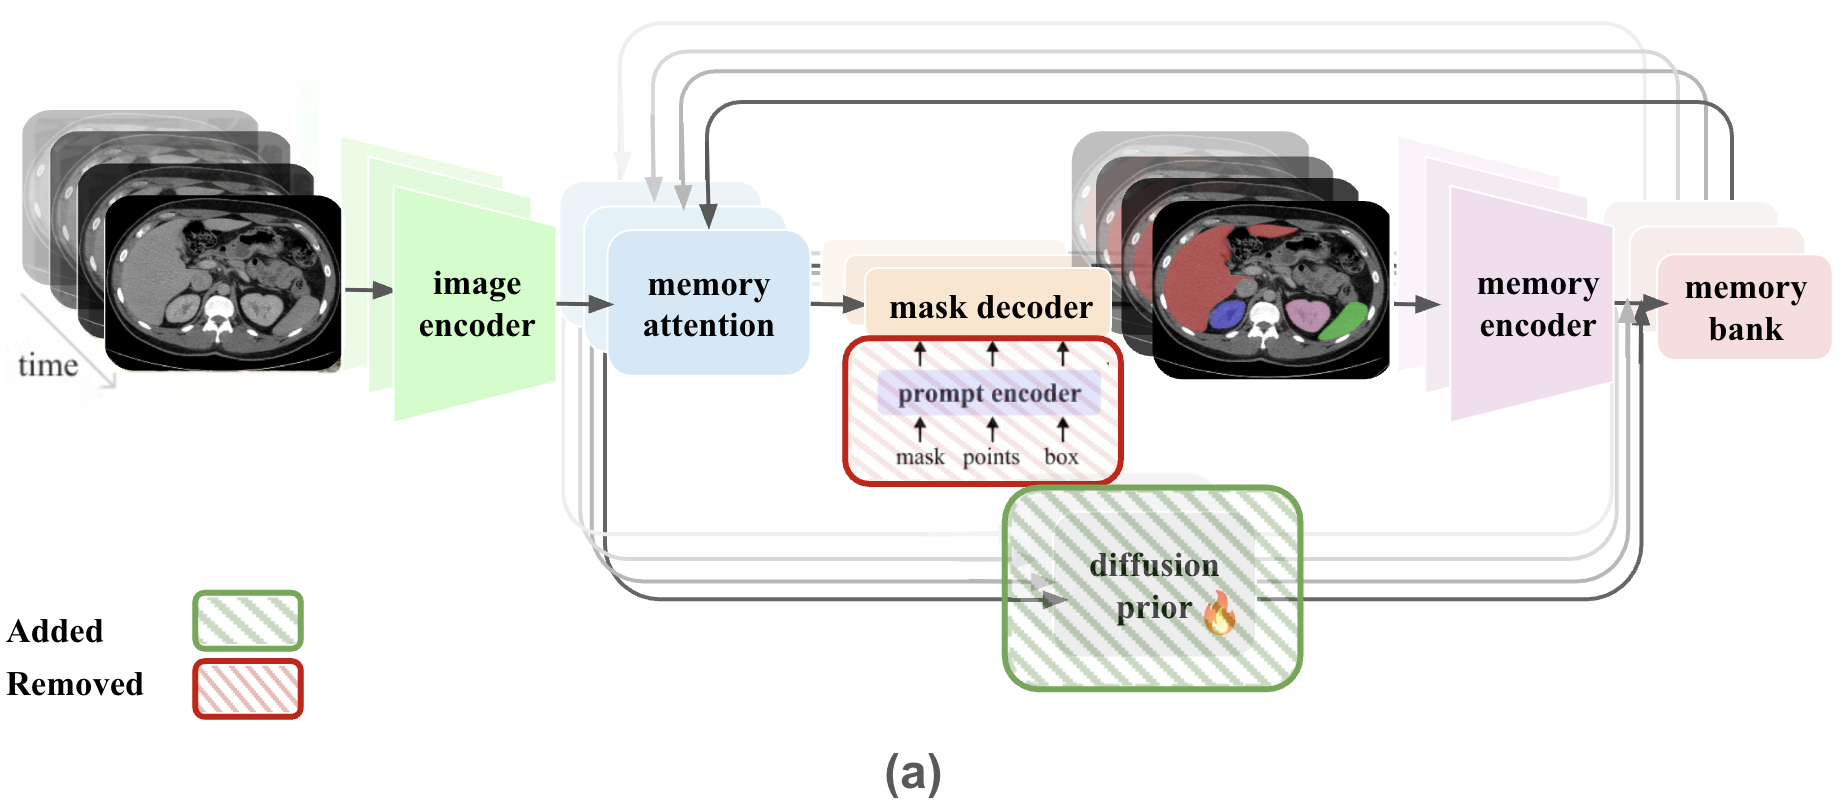
\includegraphics[width=0.8\textwidth]{pipeline_a_a.png}\hfill
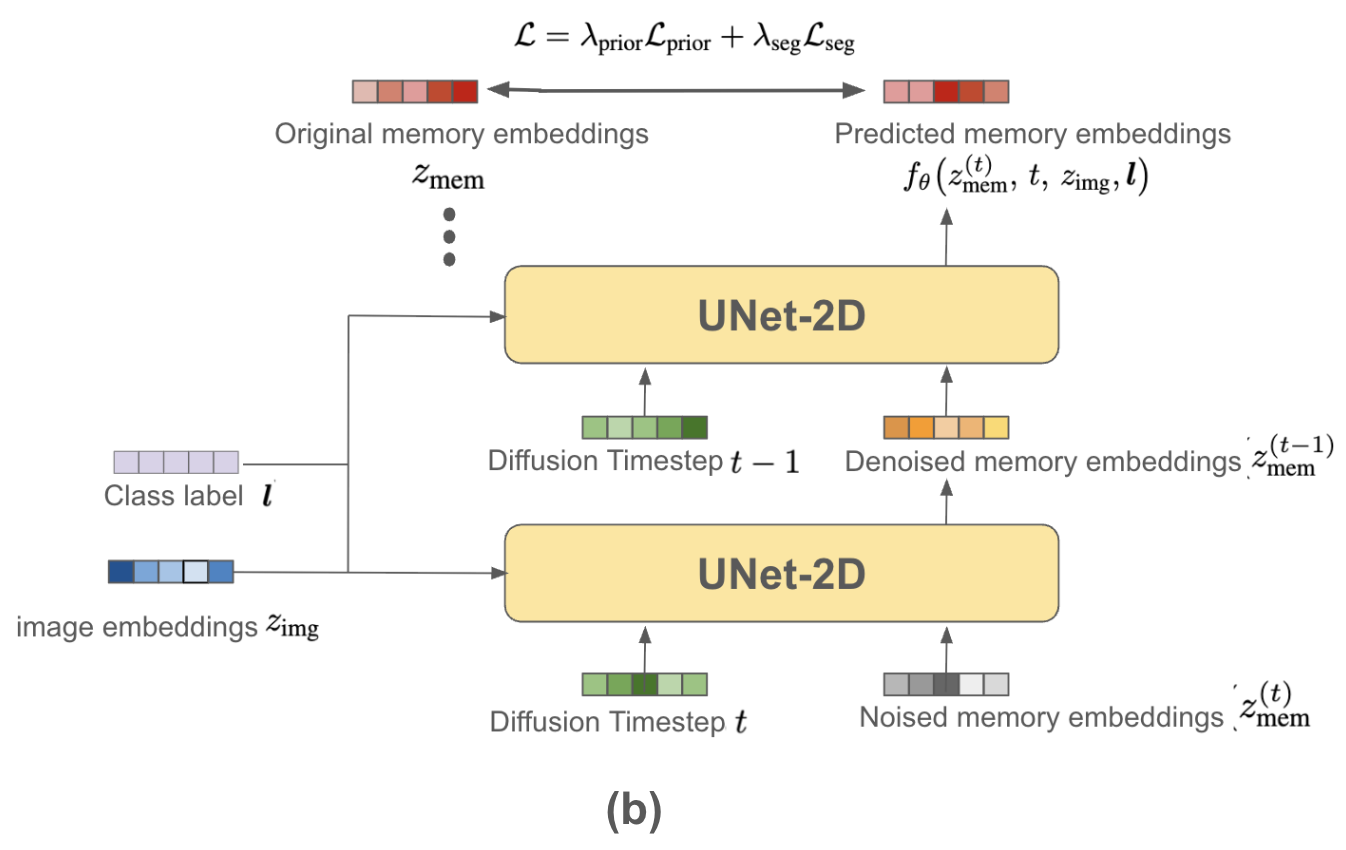
\includegraphics[width=0.6\textwidth]{pipeline_b.png}
\caption{Outline of DiffuSAM. (a)~A diffusion prior (green) generates memory embeddings from SAM2 image encoder features, eliminating the need for user prompts (red). All SAM2 components remain frozen during training. (b)~Diffusion prior model: during training it takes a noised memory embedding, image embedding, timestep embedding, and class label, and learns to denoise; at inference it generates memory from pure noise in 2 steps.}
\label{fig:pipeline}
\end{figure}

\bigskip

% --- Figure 2: t-SNE visualizations ---
\begin{figure}[ht]
\centering
\begin{minipage}[t]{0.48\textwidth}
  \centering
  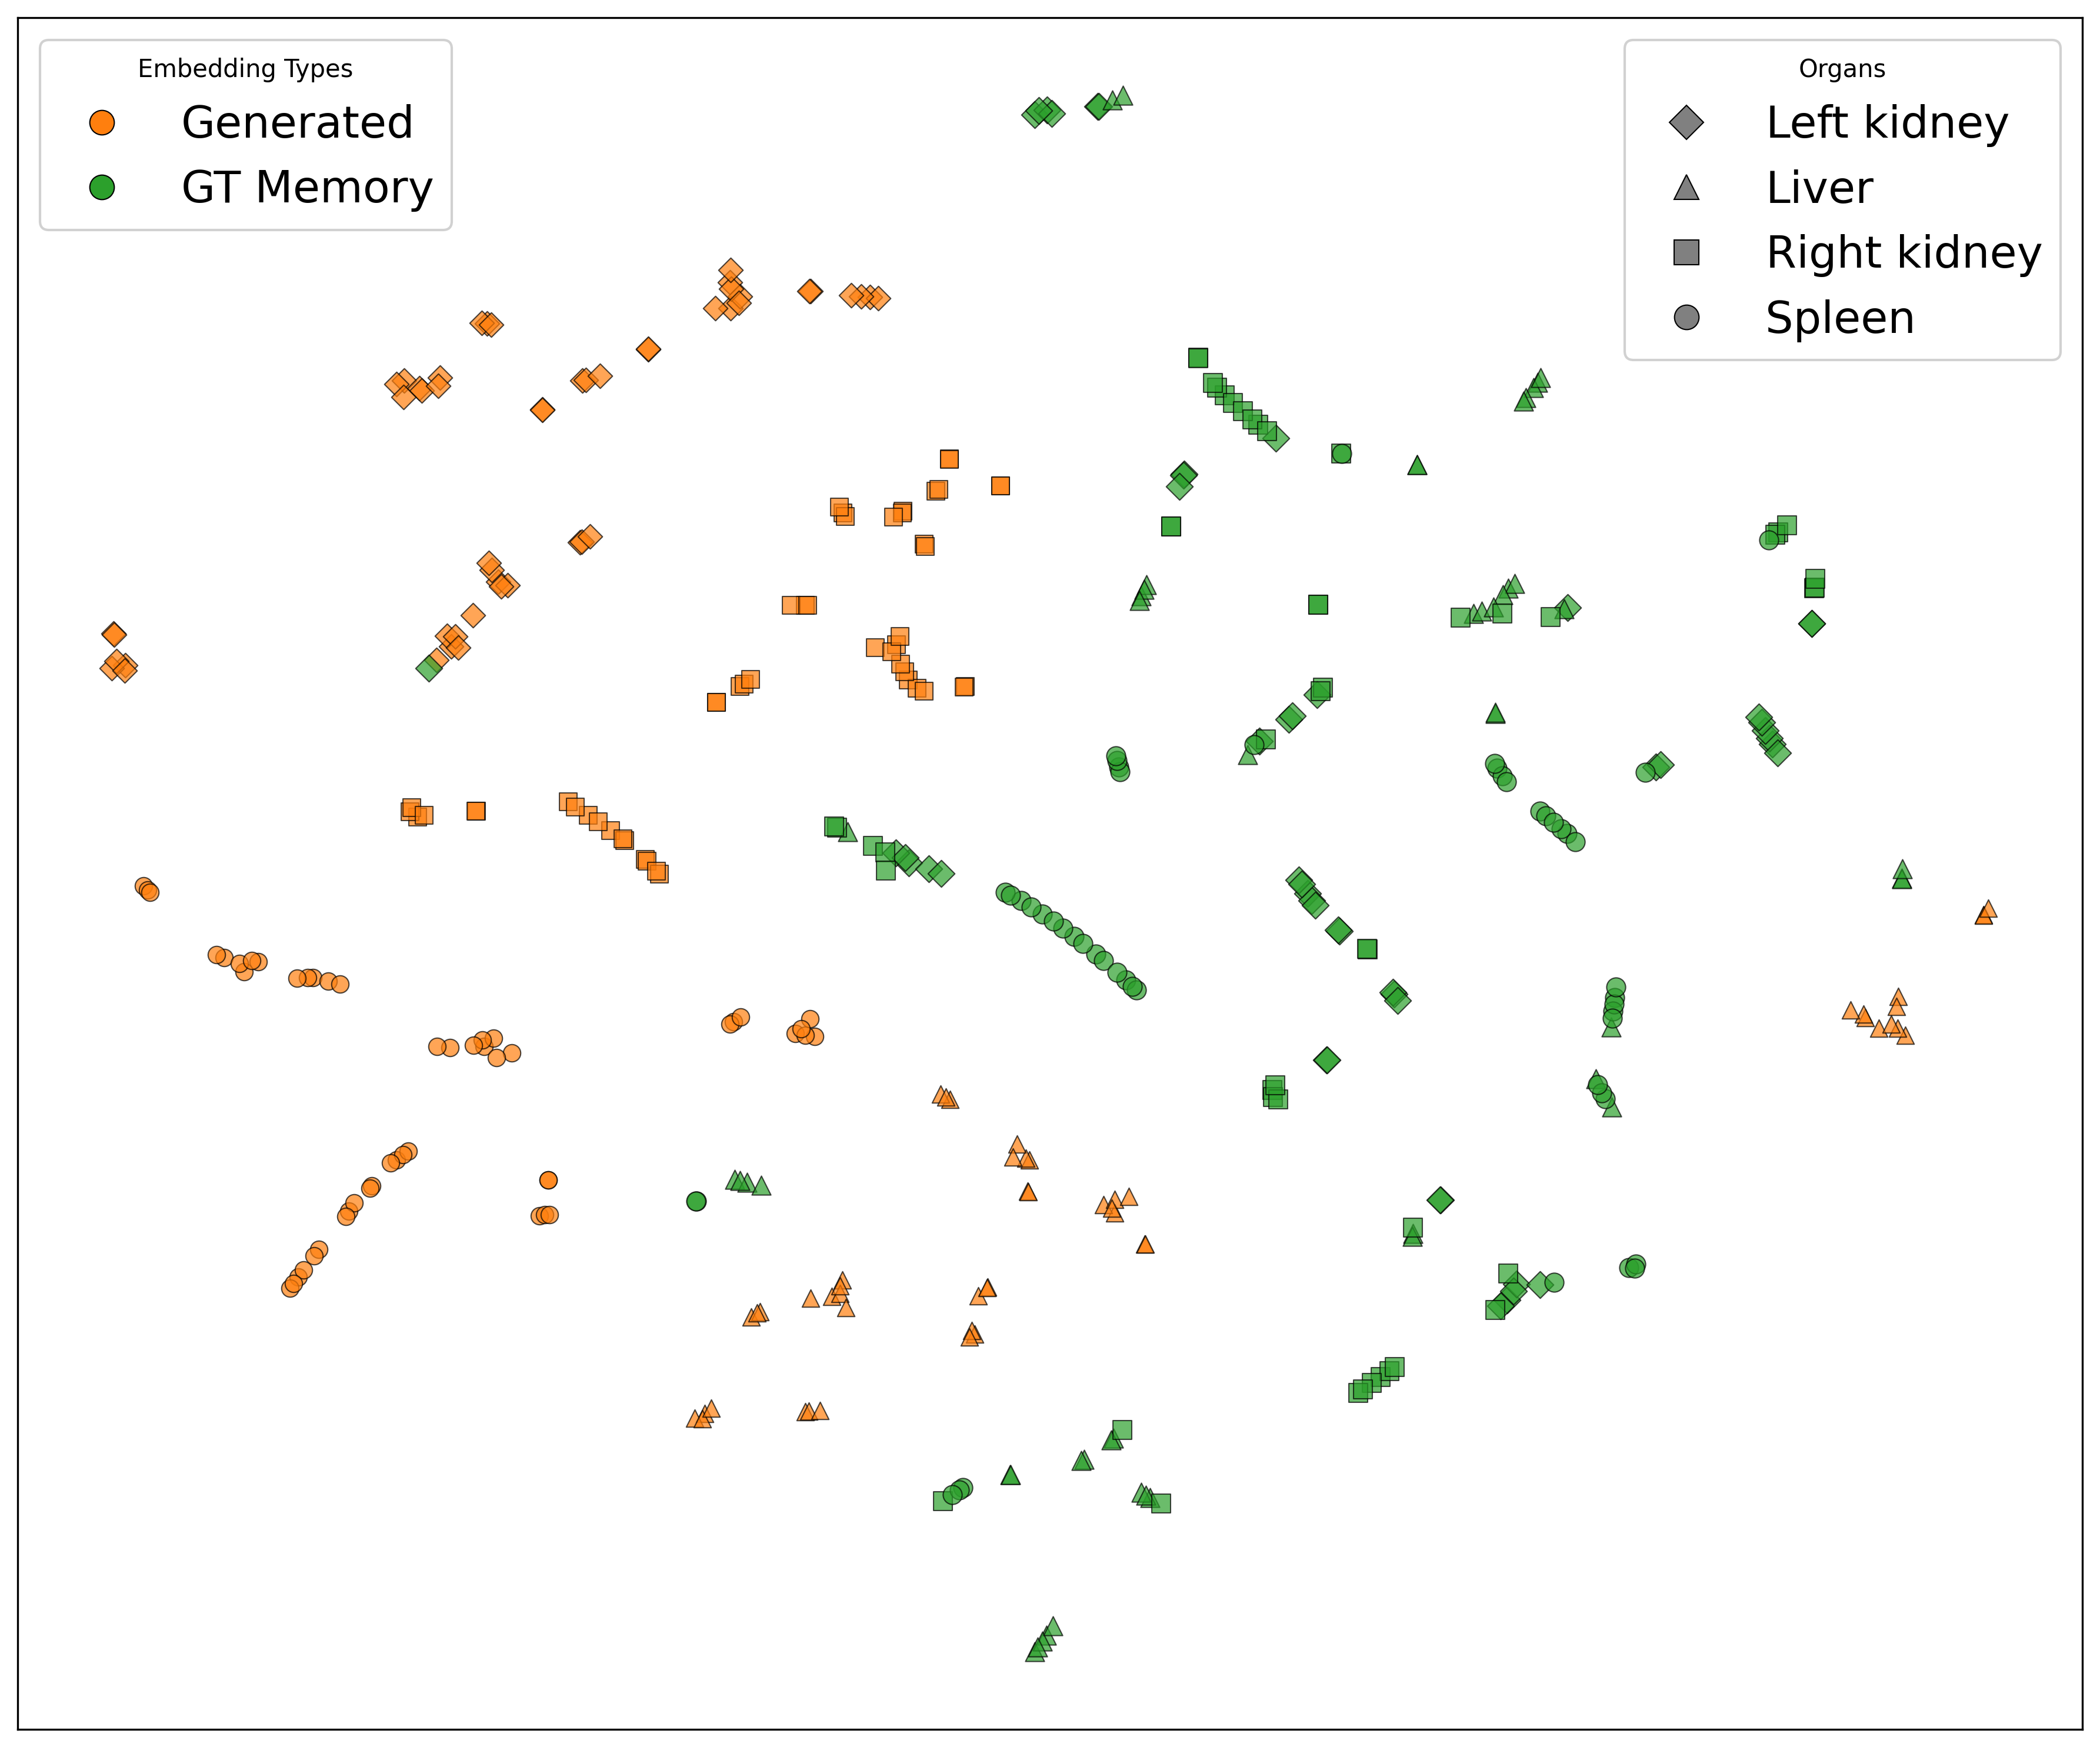
\includegraphics[width=\textwidth]{tsne_combined_all_organs_perp3_epoch1.png}\\[2pt]
  {\small (A) Early training (epoch 1)}
\end{minipage}\hfill
\begin{minipage}[t]{0.48\textwidth}
  \centering
  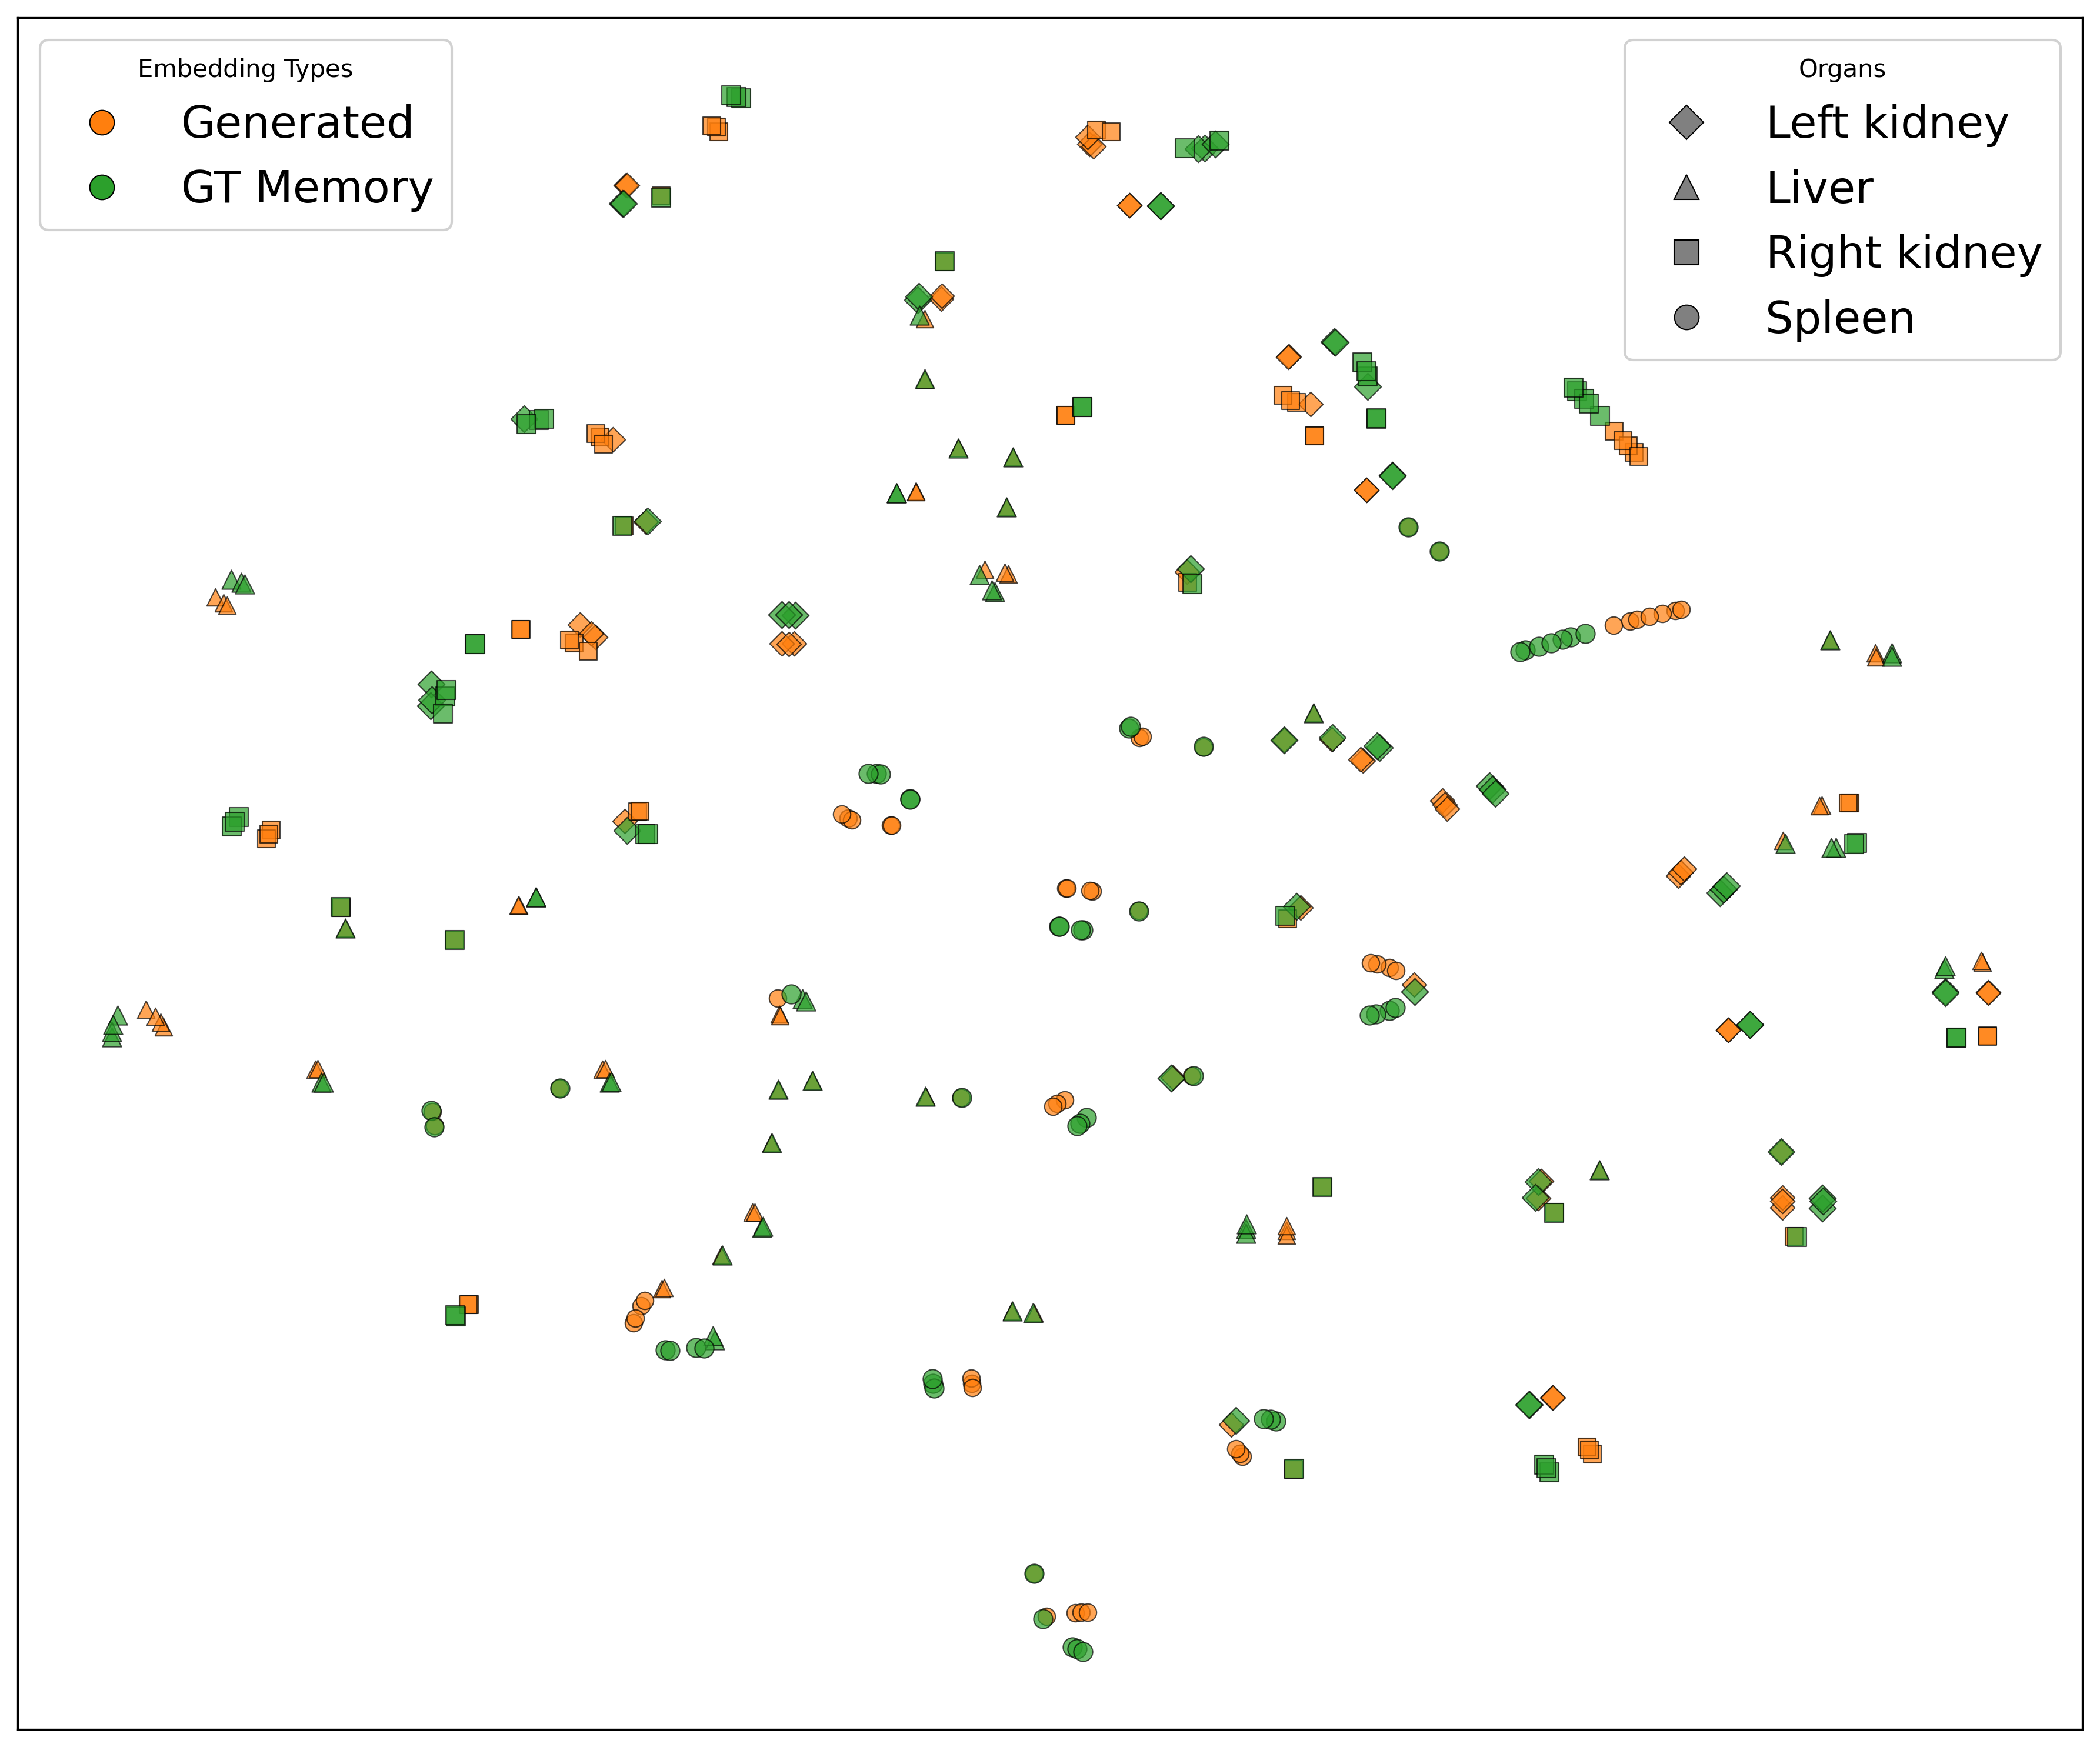
\includegraphics[width=\textwidth]{tsne_combined_all_organs_perp3_epoch75.png}\\[2pt]
  {\small (B) End of training (epoch 75)}
\end{minipage}
\caption{t-SNE of diffusion-generated vs.\ ground-truth SAM2 memory embeddings. (A)~Early training: diffuse, misaligned clusters. (B)~End of training: compact clusters aligned with ground truth.}
\label{fig:tsne}
\end{figure}

\bigskip

% --- Figure 3: Inference steps ---
\begin{figure}[ht]
\centering
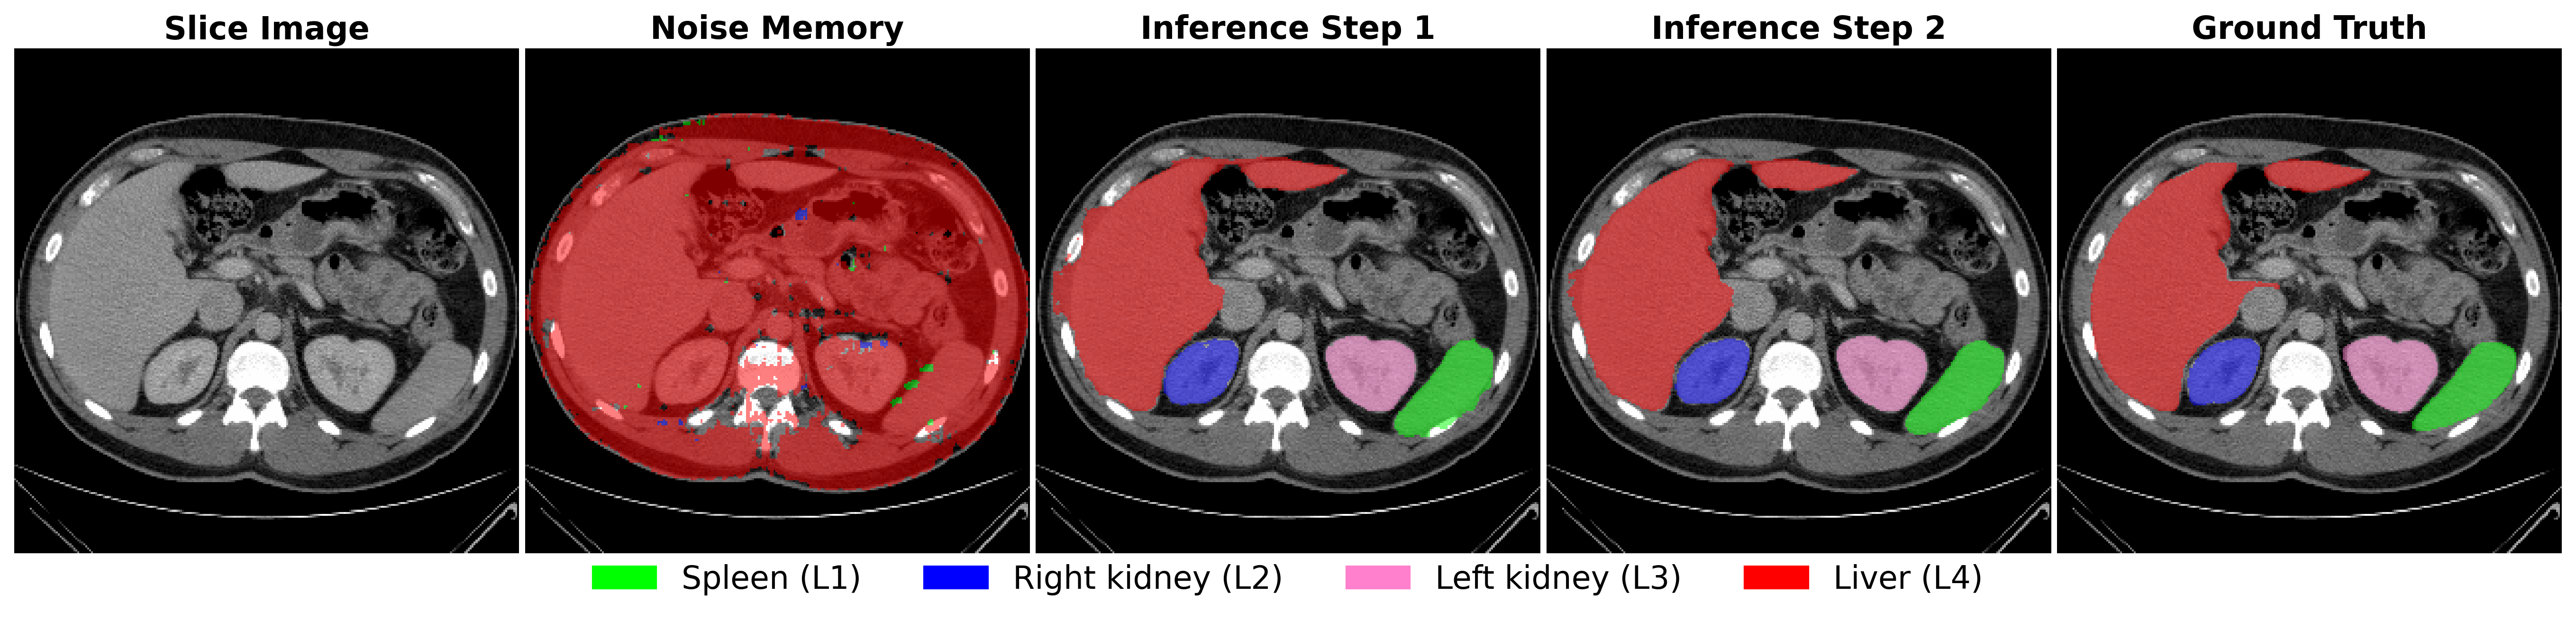
\includegraphics[width=0.9\textwidth]{inference_steps_patient_36_slice_32.png}\\[4pt]
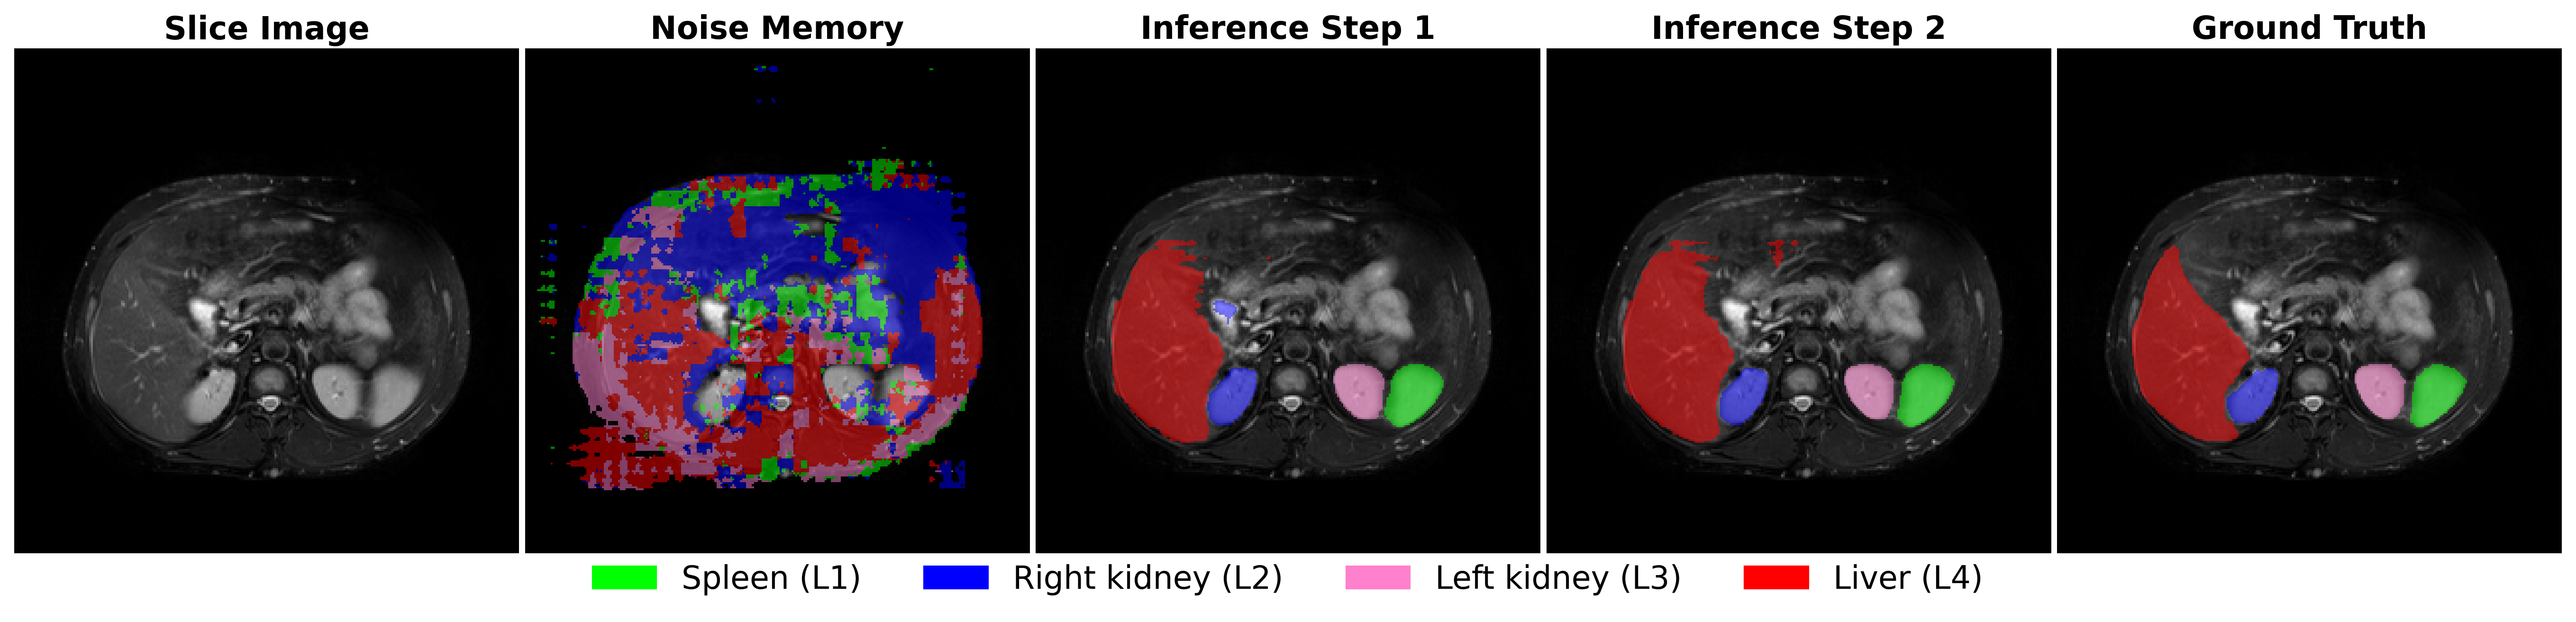
\includegraphics[width=0.9\textwidth]{inference_steps_patient_IMG-0007-2_slice_10.png}
\caption{Progressive refinement during diffusion inference. Top: CT (BTCV). Bottom: MRI (CHAOS). The model converges to accurate segmentations in 2 diffusion steps.}
\label{fig:inference-steps}
\end{figure}

% --- Table 1: Few-shot results ---
\begin{table}[h!]
\centering
\caption{Few-shot Dice scores (\%) per organ on the BTCV dataset (3 training volumes).}
\label{tab:fewshot}
\begin{tabular}{lccccc}
\toprule
Method & Spleen & R.Kidney & L.Kidney & Liver & \textbf{Avg} \\
\midrule
UNet~[4]      & 54.85 & 55.99 & 48.70 & 85.85 & 61.35 \\
UNETR~[5]     &  8.65 &  0.24 &  2.14 & 78.15 & 22.30 \\
SAM~[1]       & 15.53 & 52.19 & 62.19 & 26.56 & 39.12 \\
SAM2~[2]      & 20.24 & 55.67 & 66.94 & 34.59 & 44.36 \\
FATE-SAM~[6]  & 86.22 & \textbf{90.99} & \textbf{89.32} & 82.17 & 87.18 \\
\midrule
DiffuSAM (w/o 3D) & 82.87 & 80.95 & 83.56 & 83.49 & 82.72 \\
\textbf{DiffuSAM}  & \textbf{86.54} & 88.61 & 86.50 & \textbf{87.29} & \textbf{87.24} \\
\bottomrule
\end{tabular}
\end{table}

\bigskip

% --- Table 2: SF-UDA results ---
\begin{table}[h!]
\centering
\caption{SF-UDA Dice scores (\%) per organ (Source: BTCV CT $\to$ Target: CHAOS MRI).}
\label{tab:sfuda}
\begin{tabular}{lccccc}
\toprule
Method & Spleen & R.Kidney & L.Kidney & Liver & \textbf{Avg} \\
\midrule
Target-supervised & 94.50 & 95.50 & 95.30 & 95.10 & 95.10 \\
DPL~[8]           & 38.30 & 65.30 & 57.30 & 63.10 & 56.00 \\
DFG~[7]           & \textbf{85.10} & \textbf{92.50} & 79.60 & \textbf{83.60} & \textbf{85.20} \\
\midrule
DiffuSAM (w/o 3D) & 76.30 & 85.80 & 85.20 & 74.30 & 80.40 \\
\textbf{DiffuSAM}  & 84.60 & 87.69 & \textbf{86.29} & 82.20 & \textbf{85.20} \\
\bottomrule
\end{tabular}
\end{table}

\end{document}
